\chapter{电势与电容}

本章围绕电势、电势差、电容与电场能量展开，题目按高考、竞赛与大学物理三个层次组织，并补充两道开放性讨论题。解题中统一使用电势的叠加原理、线积分定义
\[
V(B)-V(A)=-\int_A^B \vb*{E}\cdot \dd{\vb*{l}},
\]
以及电场能量表达式
\[
W=\frac12 CU^2=\frac12 QU=\int \frac{\varepsilon E^2}{2}\,\dd{\tau}.
\]

\begin{gaokao}
在点电荷 $+Q$ 的电场中，取过该点电荷的若干球面作为等势面。已知半径分别为 $r_1,r_2,r_3$，且 $r_1<r_2<r_3$。

\begin{center}
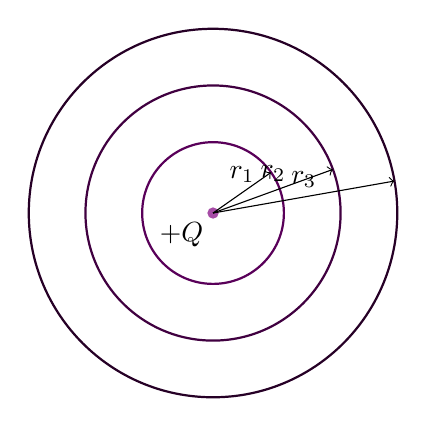
\begin{tikzpicture}[scale=0.9]
  \fill[violet!70] (0,0) circle (0.08);
  \node[below left] at (0,0) {$+Q$};
  \draw[thick,violet!70!black] (0,0) circle (1.0);
  \draw[thick,violet!50!black] (0,0) circle (1.8);
  \draw[thick,violet!30!black] (0,0) circle (2.6);
  \draw[->] (0,0) -- (35:1.0) node[midway,above] {$r_1$};
  \draw[->] (0,0) -- (20:1.8) node[midway,above] {$r_2$};
  \draw[->] (0,0) -- (10:2.6) node[midway,above] {$r_3$};
\end{tikzpicture}
\end{center}

求：
\begin{enumerate}
  \item 三个球面上的电势大小关系；
  \item 将试探电荷 $+q$ 从 $r_1$ 移到 $r_3$ 时电场力所做的功；
  \item 说明为什么电场线与等势面处处垂直。
\end{enumerate}

\begin{solution}
点电荷的电势为
\[
V(r)=\frac{1}{4\pi\varepsilon_0}\frac{Q}{r}.
\]
因此
\[
V_1>V_2>V_3.
\]
把试探电荷 $+q$ 从 $r_1$ 移到 $r_3$，电场力做功
\[
W=q(V_1-V_3)=\frac{Qq}{4\pi\varepsilon_0}\qty(\frac{1}{r_1}-\frac{1}{r_3}).
\]
若等势面上存在切向电场分量 $E_t$，则电荷沿等势面移动时有
\[
\dd{W}=q\vb*{E}\cdot \dd{\vb*{l}}=qE_t\dd{l}\neq 0,
\]
这与“等势面上移动电荷电场力不做功”矛盾，所以 $E_t=0$，故电场线必与等势面垂直。
\end{solution}
\end{gaokao}

\begin{gaokao}
如图所示，一只电容为 $C$ 的平行板电容器通过电阻 $R$ 与电动势为 $\mathcal{E}$ 的电源相连，开关闭合后开始充电。设初始时电容器不带电。

\begin{center}
\begin{circuitikz}[american voltages]
  \draw (0,0) to[battery1,l=$\mathcal{E}$] (0,3)
        to[switch,l=$S$] (2,3)
        to[R,l=$R$] (4,3)
        to[C,l=$C$] (4,0) -- (0,0);
\end{circuitikz}
\end{center}

已知某时刻电容器两端电压为 $U$。
\begin{enumerate}
  \item 写出此时电路中的电流 $I$；
  \item 求此时电容器所带电荷量 $Q$；
  \item 求从开始到该时刻电源提供的总能量中，有多少转化为电容器储能。
\end{enumerate}

\begin{solution}
闭合电路中电阻两端电压为 $\mathcal{E}-U$，由欧姆定律得
\[
I=\frac{\mathcal{E}-U}{R}.
\]
电容器所带电荷量
\[
Q=CU.
\]
电容器储存的电场能量为
\[
W_C=\frac12 CU^2.
\]
从开始到该时刻，电源输出电荷量就是电容器极板上累积的电荷量 $Q=CU$，故电源提供能量
\[
W_{\text{源}}=\mathcal{E}Q=\mathcal{E}CU.
\]
于是其中转化为电容器储能的部分占
\[
\eta=\frac{W_C}{W_{\text{源}}}=\frac{U}{2\mathcal{E}},
\]
对应的能量就是 $\frac12 CU^2$，其余部分在电阻上转化为焦耳热。
\end{solution}
\end{gaokao}

\begin{gaokao}
两块面积为 $S$、板间距为 $d$ 的平行板电容器接在恒压电源 $U$ 上，忽略边缘效应与介质影响。请不用结论 $W=\frac12 CU^2$，而是从“逐步搬运电荷”的微积分观点重新求出电容器中储存的电场能量。

\begin{solution}
平行板电容器的电容
\[
C=\frac{\varepsilon_0 S}{d}.
\]
设充电过程中某时刻已带电量为 $q$，此时两板间电势差为
\[
u=\frac{q}{C}.
\]
再搬运微元电荷 $\dd{q}$ 从负板到正板，外界至少要做功
\[
\dd{W}=u\,\dd{q}=\frac{q}{C}\dd{q}.
\]
总能量为
\[
W=\int_0^Q \frac{q}{C}\dd{q}=\frac{Q^2}{2C}.
\]
又因为最终 $Q=CU$，故
\[
W=\frac12 CU^2.
\]
若代入平行板电容器的电容，可得
\[
W=\frac12 \frac{\varepsilon_0 S}{d}U^2.
\]
这个积分过程说明：电容器储能本质上来自对不断增强的电场做功。
\end{solution}
\end{gaokao}

\begin{competition}
空间中固定有三个点电荷：在正三角形三个顶点上分别放置 $q,q,-2q$，边长为 $a$。取无穷远处电势为零。
\begin{enumerate}
  \item 求三角形中心 $O$ 处的电势；
  \item 求将试探电荷 $Q_0$ 从无穷远移到 $O$ 点时外力做功；
  \item 讨论若把 $-2q$ 改为 $-q$，中心处电势会发生什么变化。
\end{enumerate}

\begin{solution}
正三角形中心到三个顶点的距离均为
\[
R=\frac{a}{\sqrt{3}}.
\]
电势满足标量叠加，因此
\[
V_O=\frac{1}{4\pi\varepsilon_0}\qty(\frac{q}{R}+\frac{q}{R}-\frac{2q}{R})=0.
\]
故把试探电荷 $Q_0$ 从无穷远移到中心时，外力做功
\[
W_{\text{外}}=Q_0(V_O-0)=0.
\]
若将 $-2q$ 改为 $-q$，则总电荷代数和变为 $q$，中心处电势为
\[
V_O'=\frac{1}{4\pi\varepsilon_0}\frac{q}{R}
=\frac{\sqrt{3}q}{4\pi\varepsilon_0 a},
\]
不再为零。这个例子说明：尽管中心处对称性很强，但电势只取决于各点电荷电势的代数和，而非电场是否互相抵消。
\end{solution}
\end{competition}

\begin{competition}
内半径为 $a$、外半径为 $b$ 的球形电容器由两个同心导体球壳构成，中间充满真空，内球壳带电量 $+Q$，外球壳带电量 $-Q$。
\begin{enumerate}
  \item 用高斯定理求两球壳间的场强；
  \item 通过积分求内外球壳间电势差；
  \item 写出该球形电容器的电容。
\end{enumerate}

\begin{solution}
在 $a<r<b$ 的区域取半径为 $r$ 的球面作高斯面，有
\[
E\cdot 4\pi r^2=\frac{Q}{\varepsilon_0},
\]
故
\[
E(r)=\frac{Q}{4\pi\varepsilon_0 r^2}.
\]
内球壳相对外球壳的电势差为
\[
U=V_a-V_b=\int_b^a \vb*{E}\cdot \dd{\vb*{l}}
=\int_a^b \frac{Q}{4\pi\varepsilon_0 r^2}\dd{r}
=\frac{Q}{4\pi\varepsilon_0}\qty(\frac{1}{a}-\frac{1}{b}).
\]
因此电容
\[
C=\frac{Q}{U}=4\pi\varepsilon_0\frac{ab}{b-a}.
\]
当 $b\to \infty$ 时，可退化为孤立导体球的电容 $C=4\pi\varepsilon_0 a$。
\end{solution}
\end{competition}

\begin{competition}
有三个电容器，电容分别为 $C,2C,3C$。先将 $C$ 与 $2C$ 串联后，再与 $3C$ 并联接在电压为 $U$ 的电源上。
\begin{enumerate}
  \item 求总电容；
  \item 求每个电容器储存的能量；
  \item 证明总能量等于各部分能量之和，并比较串联支路与并联支路的储能差异。
\end{enumerate}

\begin{solution}
串联支路等效电容
\[
C_s=\frac{C\cdot 2C}{C+2C}=\frac{2}{3}C.
\]
再与 $3C$ 并联，总电容
\[
C_{\text{eq}}=C_s+3C=\frac{11}{3}C.
\]
串联支路两端电压也是 $U$，其带电量
\[
Q_s=C_sU=\frac{2}{3}CU.
\]
于是串联中电容 $C$ 上电压
\[
U_1=\frac{Q_s}{C}=\frac{2}{3}U,
\qquad
U_2=\frac{Q_s}{2C}=\frac{1}{3}U.
\]
各自能量为
\[
W_1=\frac12 C\qty(\frac{2}{3}U)^2=\frac{2}{9}CU^2,
\qquad
W_2=\frac12 (2C)\qty(\frac{1}{3}U)^2=\frac{1}{9}CU^2.
\]
并联支路中 $3C$ 直接承受电压 $U$，故
\[
W_3=\frac12\cdot 3C\cdot U^2=\frac{3}{2}CU^2.
\]
总能量
\[
W_{\text{总}}=W_1+W_2+W_3=\frac{11}{6}CU^2
=\frac12 C_{\text{eq}}U^2.
\]
可见并联支路由于电压高且电容大，储能明显占优势；串联支路中，总电压被分配后，储能相对较小。
\end{solution}
\end{competition}

\begin{university}
已知二维电场
\[
\vb*{E}(x,y)=\alpha x\,\vu{x}+\beta y\,\vu{y},
\]
其中 $\alpha,\beta$ 为常数。取原点 $O(0,0)$ 的电势为零。
\begin{enumerate}
  \item 计算点 $P(x_0,y_0)$ 的电势；
  \item 分别沿折线 $O\to(x_0,0)\to P$ 与 $O\to(0,y_0)\to P$ 积分，验证结果一致；
  \item 写出等势线方程。
\end{enumerate}

\begin{solution}
由定义
\[
V(P)-V(O)=-\int_O^P \vb*{E}\cdot \dd{\vb*{l}}.
\]
取路径一：先沿 $x$ 轴，再沿 $y$ 轴。
第一段有 $y=0$，故
\[
-\int_0^{x_0} \alpha x\,\dd{x}=-\frac12\alpha x_0^2.
\]
第二段有 $x=x_0$、$\dd{\vb*{l}}=\dd{y}\,\vu{y}$，故
\[
-\int_0^{y_0} \beta y\,\dd{y}=-\frac12\beta y_0^2.
\]
因此
\[
V(x_0,y_0)=-\frac12\alpha x_0^2-\frac12\beta y_0^2.
\]
若沿路径二积分，得到的也是相同结果，因为该电场满足
\[
\pdv{E_x}{y}=0=\pdv{E_y}{x},
\]
是保守场。等势线满足
\[
\alpha x^2+\beta y^2=\text{常量}.
\]
当 $\alpha,\beta>0$ 时，这是一族椭圆。
\end{solution}
\end{university}

\begin{university}
一段长度为 $L$ 的同轴电缆，内导体半径为 $a$，外导体内半径为 $b$，中间充满介电常数为 $\varepsilon$ 的均匀介质。求其电容，并说明为什么工程上常用同轴结构传输信号。

\begin{center}
\begin{tikzpicture}[scale=1.0]
  \draw[fill=gray!35] (0,0) circle (0.45);
  \draw[thick] (0,0) circle (1.4);
  \draw[thick] (0,0) circle (1.9);
  \node at (0,0) {内导体};
  \node at (0,1.65) {外导体};
  \draw[->] (0,0) -- (0.45,0) node[midway,below] {$a$};
  \draw[->] (0,0) -- (1.4,0) node[midway,below] {$b$};
\end{tikzpicture}
\end{center}

\begin{solution}
设内导体单位长度带电量为 $\lambda$。在 $a<r<b$ 的圆柱面上，由高斯定理得
\[
E(r)\cdot 2\pi rL=\frac{\lambda L}{\varepsilon},
\qquad
E(r)=\frac{\lambda}{2\pi\varepsilon r}.
\]
内外导体间电势差为
\[
U=\int_a^b E(r)\dd{r}=\frac{\lambda}{2\pi\varepsilon}\ln\frac{b}{a}.
\]
总电荷量 $Q=\lambda L$，故电容
\[
C=\frac{Q}{U}=\frac{2\pi\varepsilon L}{\ln(b/a)}.
\]
同轴结构的优点在于：
\begin{enumerate}
  \item 电场主要限制在两导体之间，外部辐射小；
  \item 结构对称，参数稳定，便于计算特性阻抗和单位长度电容；
  \item 抗外界电磁干扰能力强，适合高频信号传输。
\end{enumerate}
\end{solution}
\end{university}

\begin{university}
设一平行板电容器面积为 $S$，板间距为 $d$，两板间充满介电常数为 $\varepsilon$ 的均匀介质，两板电势差为 $U$。请从电场能量密度
\[
w=\frac12\varepsilon E^2
\]
出发，直接积分求总储能，并与 $\frac12 CU^2$ 对照验证。

\begin{solution}
忽略边缘效应时，板间场强近似均匀，
\[
E=\frac{U}{d}.
\]
电场能量密度
\[
w=\frac12\varepsilon \frac{U^2}{d^2}.
\]
场所在体积为
\[
\tau=Sd.
\]
所以总能量
\[
W=\int w\,\dd{\tau}=wSd=\frac12\varepsilon \frac{U^2}{d^2}Sd
=\frac12\frac{\varepsilon S}{d}U^2.
\]
而平行板电容器电容为
\[
C=\frac{\varepsilon S}{d},
\]
故
\[
W=\frac12 CU^2.
\]
这说明宏观电容储能公式与微观能量密度积分是完全一致的。
\end{solution}
\end{university}

\begin{problem}
两极板面积为 $S$、间距为 $d$ 的电容器中填充了分层非均匀介质：左半区域介电常数为 $\varepsilon_1$，右半区域介电常数为 $\varepsilon_2$，分界面与电场方向平行。
\begin{enumerate}
  \item 求等效电容；
  \item 若分界面改为与极板平行，等效电容会怎样变化；
  \item 说明“非均匀介质中的电容”为什么往往可转化为串并联模型。
\end{enumerate}

\begin{solution}
当分界面与电场方向平行时，相当于两个面积各为 $S/2$、板间距相同为 $d$ 的平行板电容器并联：
\[
C_1=\frac{\varepsilon_1 S}{2d},
\qquad
C_2=\frac{\varepsilon_2 S}{2d}.
\]
故等效电容
\[
C_{\parallel}=C_1+C_2=\frac{(\varepsilon_1+\varepsilon_2)S}{2d}.
\]
若分界面与极板平行，则相当于上下两层介质厚度各为 $d/2$ 串联：
\[
C_1'=\frac{\varepsilon_1 S}{d/2}=\frac{2\varepsilon_1 S}{d},
\qquad
C_2'=\frac{2\varepsilon_2 S}{d}.
\]
所以
\[
\frac{1}{C_{\text{串}}}=\frac{1}{C_1'}+\frac{1}{C_2'}
=\frac{d}{2S}\qty(\frac{1}{\varepsilon_1}+\frac{1}{\varepsilon_2}),
\]
即
\[
C_{\text{串}}=\frac{2\varepsilon_1\varepsilon_2 S}{(\varepsilon_1+\varepsilon_2)d}.
\]
之所以能转化为串并联模型，是因为不同区域要么承受相同电压（并联特征），要么通过相同电荷通量（串联特征），从而可用等效电路处理复杂介质分布。
\end{solution}
\end{problem}

\begin{problem}
平行板电容器的公式 $C=\varepsilon S/d$ 建立在“忽略边缘效应”的近似下。请定性分析边缘效应对以下物理量的影响：
\begin{enumerate}
  \item 实际电场分布；
  \item 实际电容与理想公式的偏差；
  \item 电容器储能和局部击穿风险。
\end{enumerate}
并说明为什么当 $d\ll \sqrt{S}$ 时该近似较好。

\begin{solution}
边缘处电场线会向外弯曲，不再与极板严格垂直，故电场不再是完全均匀场。由此带来三个直接后果：
\begin{enumerate}
  \item 有效储能体积略大于理想模型中的 $Sd$，因为部分场延伸到极板外侧；
  \item 在相同电势差下，可容纳的总电荷略多，因此实际电容通常略大于 $\varepsilon S/d$；
  \item 边缘附近场强可能局部增强，尤其在尖角或毛刺位置更明显，因此更容易先发生局部放电或介质击穿。
\end{enumerate}
当 $d\ll \sqrt{S}$ 时，极板中央的大部分区域离边界很远，中央近似均匀场占主导，边缘畸变仅局限于很窄区域，因此理想公式误差较小。工程上常通过增大极板尺寸、采用圆滑边缘和加护环等方法减弱边缘效应。
\end{solution}
\end{problem}
